\documentclass{article}
\usepackage[utf8]{inputenc}

\title{EE2703: Assignment 4}
\author{Yogesh Agarwala \\ EE19B130}
\date{March 10, 2021}

\usepackage{natbib}
\usepackage{graphicx}
\usepackage{listings}
\usepackage{amsmath}
\usepackage{subfig}

\begin{document}

\maketitle

\section{Introduction}
We will fit two functions, $e^x$ and $cos(cos(x))$ over the interval $[0,2\pi)$ using their computed fourier series coefficients. The Fourier Series of a function $f(x)$ with period $2\pi$ is computed as follows:
\vspace{2mm}
\begin{equation*}
    f(x) = a_0 + \sum_{n=1}^{+\infty}\{ a_ncos(nx) +b_nsin(nx)\}
\end{equation*}
\vspace{2mm}
where the coefficients are given by, 


\[a_0 = \frac{1}{2\pi} \int_0^{2\pi}f(x)dx\]
\[a_n = \frac{1}{\pi} \int_0^{2\pi}f(x)\cos(nx)dx\]
\[b_n = \frac{1}{\pi} \int_0^{2\pi}f(x)\sin(nx)dx\]
\vspace{2mm}

The function $e^x$
is ever increasing with $x$ and is non-periodic. However
for the evaluation of the Fourier series, the function is made 2$\pi$ periodic. $cos(x)$ is periodic and thus $cos(cos(x))$ is also periodic. Since $cos(-x) =
cos(x)$, the period of cos(cos(x)) is $\pi$.

\newpage
\section{Assignment}
\subsection*{Q1. Defining and Plotting the Functions}
    We need to ensure that the function can output correct values even for an
    N-dimensional vector as an input. The built-in functions in numpy can be
    used to accomplish the same :
    \lstset{language=Python}
    \lstset{frame=lines}
    \lstset{label={lst:code_direct}}
    \lstset{basicstyle=\footnotesize}
    \begin{lstlisting}
import numpy as np
def exp(x):
      	return np.exp(x)
def coscos(x) :
      	return np.cos(np.cos(x))
    \end{lstlisting}
	The above functions are plotted over the interval $[$-2$\pi$, 4$\pi$$)$ using 300 points
	sampled uniformly over this interval. The following plots are obtained :

    \begin{figure}[h!]
    \centering
    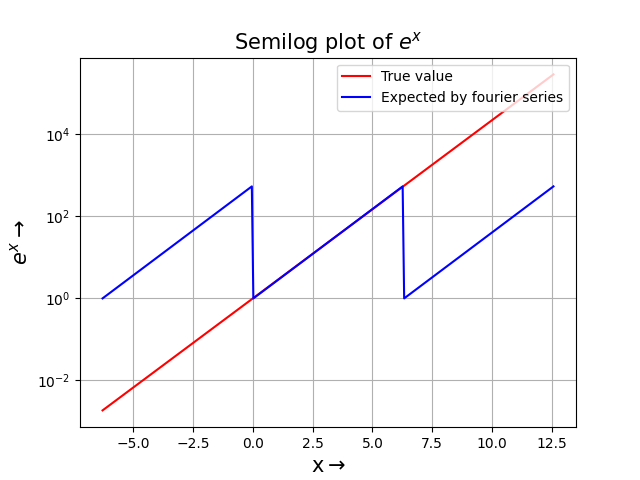
\includegraphics[scale=0.5]{q1(a)}
    \label{fig:1(a)}
    \end{figure}
\begin{figure}[h!]
	\centering
	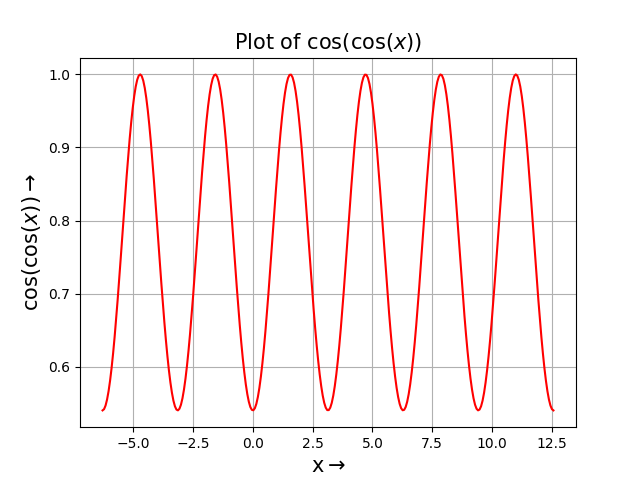
\includegraphics[scale=0.5]{q1(b)}
	\label{fig:1(b)}
\end{figure}






\subsection*{Q2. Finding the Fourier series coefficients: Integration approach}
The Fourier series coefficients are obtained using the quad function in the
scipy library. The following code snippet evaluates the first n coefficients
of the Fourier series expansion of $e^x$ and $cos(cos(x))$:


\begin{lstlisting}
func_dict = {'exp(x)':exp,'cos(cos(x))': coscos}
def find_coeff(n,label):
    coeff = np.zeros(n)
    func = func_dict[label]
    u = lambda x,k: func(x)*np.cos(k*x)
    v = lambda x,k: func(x)*np.sin(k*x)
    coeff[0]= quad(func,0,2*np.pi)[0]/(2*np.pi)
    for i in range(1,n,2):
        coeff[i] = quad(u,0,2*np.pi,args=((i+1)/2))[0]/np.pi
    for i in range(2,n,2):
        coeff[i] = quad(v,0,2*np.pi,args=(i/2))[0]/np.pi
    return coeff
\end{lstlisting}




\subsection*{Q3. Semilog and Loglog plot for both functions}
We thus obtain the first 51 coefficient of the two functions. They are saved in the following form:
\[
\begin{pmatrix}
	a_0 \\
	a_1 \\
	b_1 \\
	\dots \\
	a_{25} \\
	b_{25}
\end{pmatrix}\\
\]
\newline
Plot of the fourier coefficients of $e^x$
in semilog and loglog scale are:
\begin{figure}[h!]
	\centering
	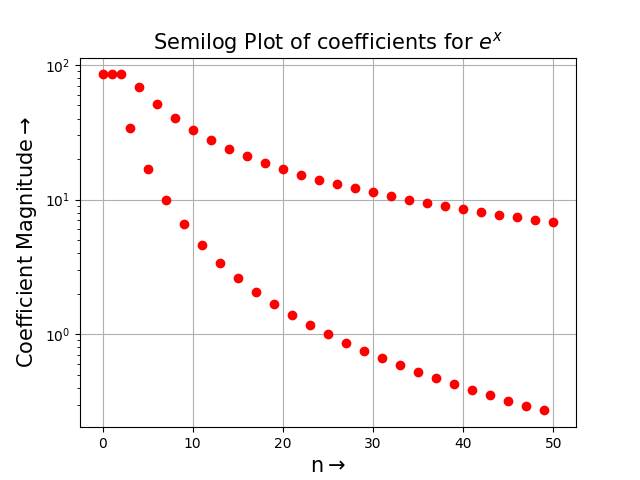
\includegraphics[scale=0.46]{q3(a)}
	\label{fig:1(b)}
\end{figure}
\begin{figure}[h!]
	\centering
	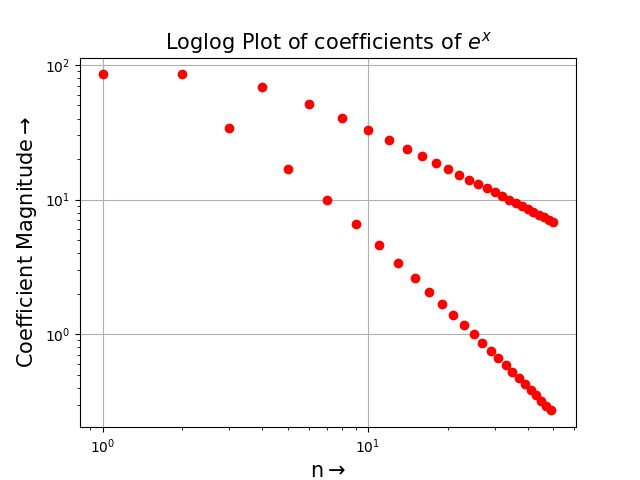
\includegraphics[scale=0.46]{q3(b)}
	\label{fig:1(b)}
\end{figure}

\newpage
Similarly, the plots for cos(cos(x)) are as follows:
\begin{figure}[h!]
	\centering
	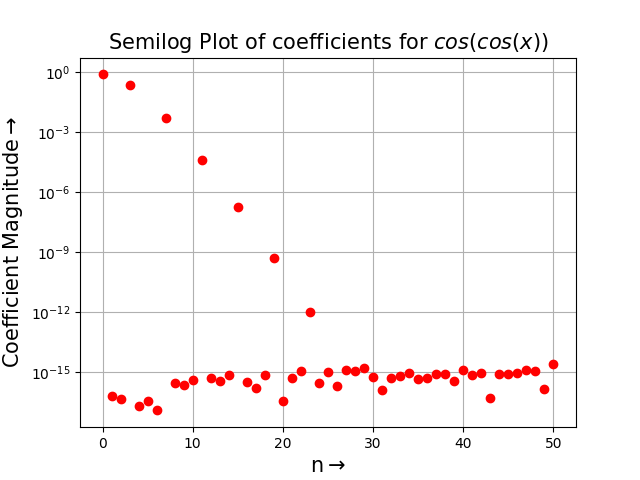
\includegraphics[scale=0.46]{q3(c)}
	\label{fig:1(b)}
\end{figure}
\begin{figure}[h!]
	\centering
	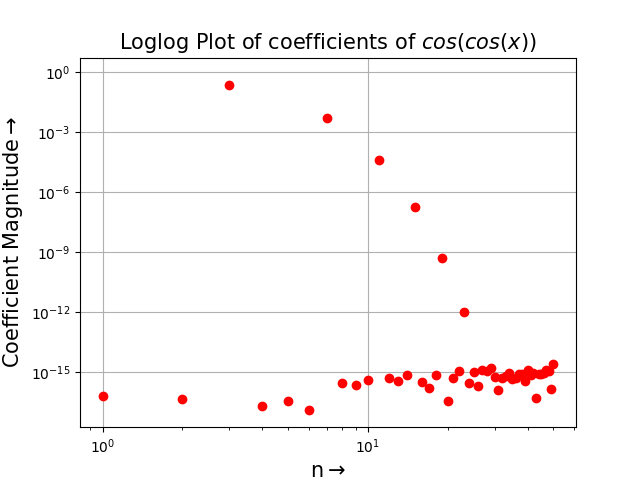
\includegraphics[scale=0.46]{q3(d)}
	\label{fig:1(b)}
\end{figure}

We notice that the $b_{n}$ coefficients in the second case are expected to be
zero as the function cos(cos(x)) is even and thus the odd sinusoidal components are zero. However, the values obtained are non-zero because of the limitation
in the numerical accuracy upto which $\pi$ can be stored in memory.

\vspace{2mm}
In the first case, the function, having an exponentially increasing gradient,
contains a wide range of frequencies in its fourier series. In the second case,
cos(cos(x)) has a relatively low frequency of $\frac{1}{\pi}$
and thus contribution by
the higher sinusoids is less, manifesting in the quick decay of the coefficients
with n.


\begin{equation}
|a_{n}|, |b_{n}| \propto \frac{1}{n^2 + 1}   
\end{equation}
Thus for large n,
\begin{equation}
log(|a_{n}|), log(|b_{n}|) \propto log(\frac{1}{n^2 + 1}) \approx -2log(n)
\end{equation}

Thus, the $loglog$ plot becomes approximately linear as n increases.
Similarly, the coefficients of cos(cos(x)) would be approximately exponential
with n . Thus the $semilog$ plot is linear.

\vspace{5mm}

\subsection*{Q4. Finding the Fourier series coefficients: "Least Squares approach"}
Building on last weeks work we now try a Least Squares Approach to this problem. We linearly choose 400 values of x in the range [0,2$\pi$). It can be Noted that far better approximations were achieved when a larger value($\sim$10000) was used instead of 400. 
We try to find the Fourier coefficients using linear regression on these 400 values. The matrix equation is\\[5mm]
\vspace{4mm}
$\begin{pmatrix} 
1 & \cos(x_1) & \sin(x_1) & .... & \cos(25x_1) & \sin(25x_1)\\
1 & \cos(x_2) & \sin(x_2) & .... & \cos(25x_2) & \sin(25x_2)\\
... & ... & ... & .... & ... & ... \\
1 & \cos(x_{400}) & \sin(x_{400}) & .... & \cos(25x_{400}) & \sin(25x_{400})
\end{pmatrix}
$$
\begin{pmatrix} 
a_0\\
a_1\\
b_1\\
...\\
a_{25}\\
b_{25}
\end{pmatrix}
=$
$
\begin{pmatrix} 
f(x_1)\\
f(x_2)\\
...\\
f(x_{400})
\end{pmatrix}\\
$
\vspace{4mm}
We create the matrix on the left side and call it \(A\).\\[-4mm]
So basically we want to solve\\
\begin{equation*}
 Ac=b
\end{equation*}
where \(c\) are the fourier coefficients.
\clearpage 

\hspace{-7mm} Code for implementing the above equation is:
\begin{lstlisting}
x = np.linspace(0,2*np.pi,401)
x = x[:-1]
A = np.zeros((400,51))
A[:,0] = 1
for i in range(1,26):
	A[:,2*i-1] = np.cos(i*x)
	A[:,2*i] = np.sin(i*x) 

b_exp = exp(x)  
b_coscos = coscos(x)

c_exp = np.linalg.lstsq(A,b_exp, rcond=None)[0]
c_coscos = np.linalg.lstsq(A,b_coscos,rcond=None)[0]

\end{lstlisting}

\vspace{5mm}

\subsection*{Comparing Runtime of Integration and Least Square approaches}

The least squares estimation method provides a faster way of evaluating a
large number of Fourier coefficients. In this case of evaluating 51 coefficients,
the time taken to evaluate the coefficients in each method are as follows:
\vspace{2mm}
\begin{lstlisting}
"""runtime: integration approach"""
start = timeit.default_timer()
coeff_exp = find_coeff(51,'exp(x)')
elapsed = timeit.default_timer() - start
print('Runtime with integration approach = ',elapsed)

"""runtime: least square approach"""
start = timeit.default_timer()
for i in range(1,26):
	A[:,2*i-1] = np.cos(i*x)
	A[:,2*i] = np.sin(i*x) 
b_exp = exp(x)  
c_exp = np.linalg.lstsq(A,b_exp, rcond=None)[0]
elapsed = timeit.default_timer() - start
print('Runtime with least square approach = ', elapsed)
\end{lstlisting}
\textbf{Code Output:}\\[2mm]Runtime with integration approach = 0.16507640000000023\\
Runtime with least square approach = 0.003682799999999986\\[4mm]
\textbf{Conclusion:}\\[1mm]
Clearly in the direct integration approach the runtime is almost
50 times the taken for the least squares approach.

\newpage
\subsection*{ Q5. Plots comparing the coefficients by "Integration" and "Least Square" approaches}

Plot of the fourier coefficients of $e^x$
in semilog and loglog scale are:

\begin{figure}[h!]
    \centering
    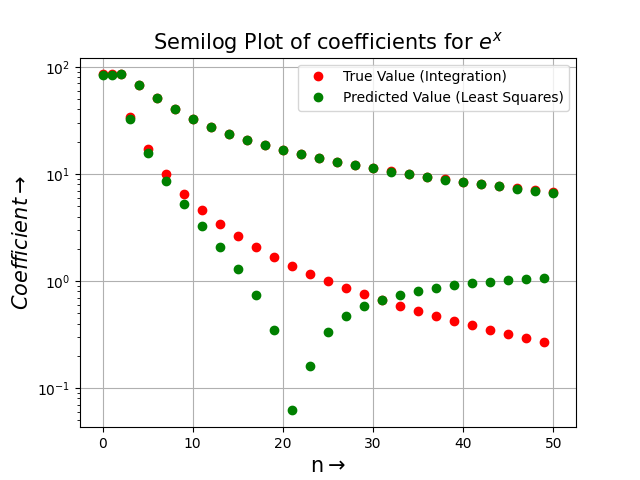
\includegraphics[scale=0.55]{q5(a)}
    \label{fig:1(b)}
\end{figure}
\begin{figure}[h!]
    \centering
    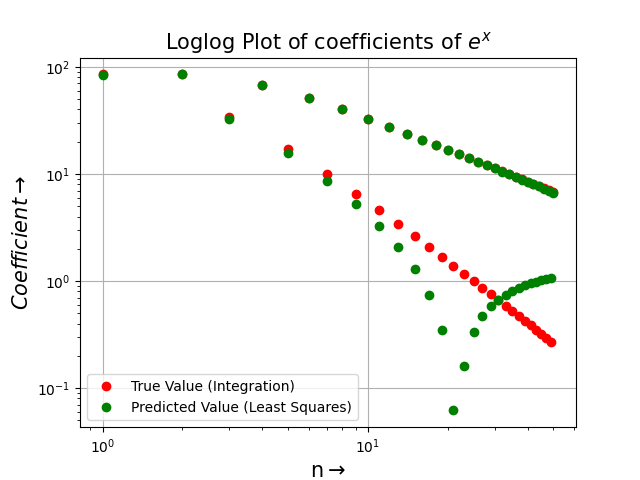
\includegraphics[scale=0.55]{q5(b)}
    \label{fig:1(b)}
\end{figure}

\newpage
Similarly, the plots for cos(cos(x)) are as follows:

\begin{figure}[h!]
    \centering
    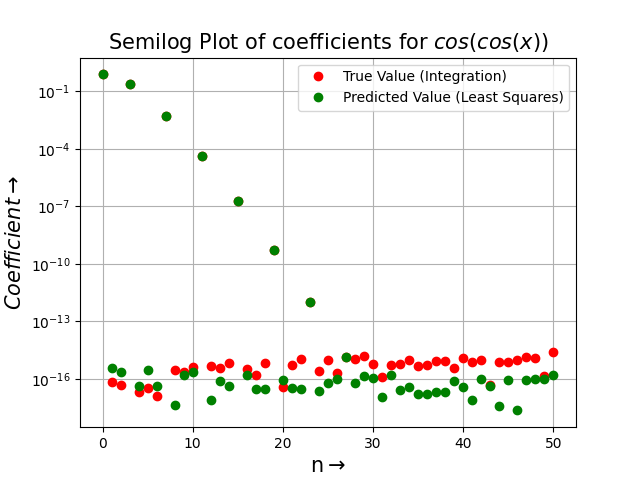
\includegraphics[scale=0.55]{q5(c)}
    \label{fig:1(b)}
\end{figure}
\begin{figure}[h!]
    \centering
    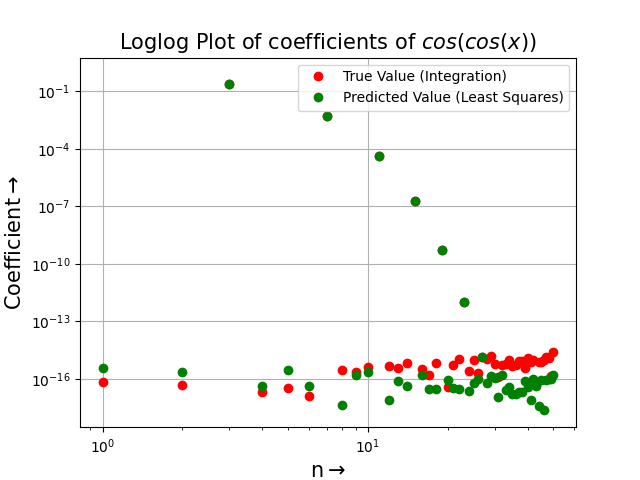
\includegraphics[scale=0.55]{q5(d)}
    \label{fig:1(b)}
\end{figure}



It can be seen that the coefficients for cos(cos(x)) are in much closer
agreement than the coefficients for $e^x$ and is also expected as the former is
periodic and the periodic extension of the latter has an increasing gradient
and would require higher sinusoids for a better representation. Since the
least squares approach is only approximate, the deviation is expected.




\clearpage
\subsection*{Q6. Calculating the deviation b/w Least square and direct integration coefficients}

\begin{lstlisting}
deviation_exp = abs(coeff_exp - c_exp)
deviation_coscos = abs(coeff_coscos - c_coscos)

max_dev_exp = np.max(deviation_exp)
max_dev_coscos = np.max(deviation_coscos)\\
\end{lstlisting}
where, coeff\_exp and coeff\_coscos are the values obtained through
integration and c\_exp and c\_coscos are the values obtained through the least
squares approach.\\
\\The maximum deviation in the coefficient of $e^x$ =1.332730870335439\newline
whereas the same metric for cos(cos(x)) = 2.674677035413032e-15\newline
Our Predictions for $e^x$ are very poor compared to that of cos(cos(x)). This can be fixed by sampling at a larger number of points.\newline 


\subsection*{Q7. Plots comparing the function values obtained by the "least squares" method with the "true" value}
The matrix product Ac gives an estimate of the function values at ${x_{1}, x_{2}, .... x_{400}}$ chosen
earlier. These estimates, along with the actual value of the functions yield
the following plots:

\begin{figure}[h!]
    \centering
    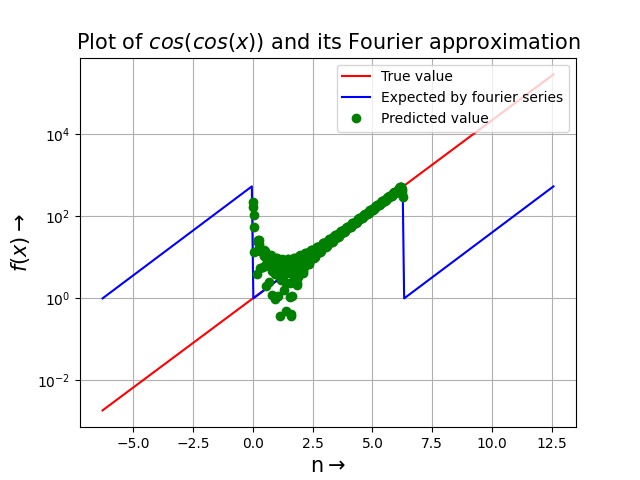
\includegraphics[scale=0.55]{q7(a).png}
    \label{fig:1(b)}
\end{figure}
\begin{figure}[h!]
    \centering
    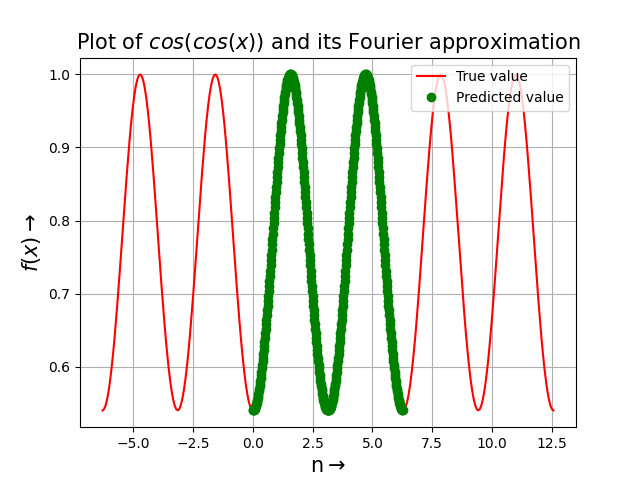
\includegraphics[scale=0.55]{q7(b).png}
    \label{fig:1(b)}
\end{figure}

\newpage

It should be noted that $e^x$ is a non periodic function and Fourier series exists only for periodic functions. Hence we have considered a variation of $e^x$ with period 2$\pi$ that has the actual value of $e^x$ only in the range [0,$2\pi$). Hence it is acceptable that there is a large discrepancy in the predicted value of $e^x$ at these boundaries.



\section{Conclusion}

The Fourier series coefficients of $e^x$ and cos(cos(x)) were found in two ways:
direct integration and estimation using the least squares approach. It was
verified that the odd sinusoidal components of cos(cos(x)) are nearly zero.
The least squares approach provided a more computationally inexpensive
way of estimating the coefficients. It was found that the least squares estimate deviated more for $e^x$
than cos(cos(x)), due to the high gradient characteristics of the former and periodic behaviour of the latter.


\end{document}
